% 作者题证的编辑转录副本，不是独立下载的上游原件。
% 来源：https://github.com/OpenLogicProject/OpenLogic/blob/master/content/model-theory/lindstrom/lindstrom-proof.tex

\paragraph{章内约定与记号（据作者定义整理）。}
语言按本章取有限关系语言并允许常量；加见证常量时使用可数扩张。
抽象逻辑为$(L,\models_L)$，其中$L(\mathcal L)$给出语言$\mathcal L$的句子。
作者称它\emph{normal}，是指满足下列条件：语言扩张时句子集合单调；每句仅依赖有限子语言；
满足关系在同构下不变；允许一致重命名符号；含原子句且对布尔运算封闭；
允许把常量量化；允许把句子相对化到由新谓词（可带参数）定义的子结构。
具体地，相对化句在大结构中成立，当且仅当原句在该定义子结构中成立。
这些条件使一阶逻辑$F$包含于$L$，并允许以下证明使用有限的编码语言。
$M\equiv_nN$表示两结构对量词秩至多$n$的一阶句子一致。
$I_n(\mathbf a,\mathbf b)$为对应的$n$步往返关系：
$I_0$表示有限元组对应保持原子公式，$I_{n+1}$要求双方每个新增元素均有对应延伸满足$I_n$。
$M\simeq_pN$表示存在非空、具有往返延伸性质的有限部分同构族。

\begin{definition}[Compactness and downward L\"owenheim--Skolem properties]
The Compactness Property says that a set $\Gamma$ of $L$-sentences is
satisfiable whenever each finite subset is satisfiable.
The downward L\"owenheim--Skolem Property says that a satisfiable theory
in a countable language has an at most countable model.
\end{definition}

\begin{theorem}[Partial isomorphisms and abstract equivalence; ls-property]
Suppose $(L,\models_L)$ is a normal logic with the L\"owenheim--Skolem
property. Any two partially isomorphic structures are elementarily
equivalent in $(L,\models_L)$.
\end{theorem}
\begin{proof}
Suppose $M\simeq_pN$, but $M\models_LE$ and $N\not\models_LE$ for some
$E$. By isomorphism invariance we may make their domains disjoint, and
by finite occurrence assume $E$ uses a finite language.
Let $\mathcal I$ witness the partial isomorphism, and assume without loss
that restrictions of members of $\mathcal I$ are again in $\mathcal I$.

Let $M^{<\omega}$ be the finite sequences from $M$. On this set let
$S(\mathbf a,\mathbf b,\mathbf c)$ express concatenation, and let
$T(\mathbf a,b,\mathbf c)$ express appending the single element $b$.
With new predicates $P,Q$ for these relations, build $M^*$ on
$M\cup M^{<\omega}$, retaining $M$ as a distinguished substructure.
Define $N^*$ in the same way.
Represent $\mathcal I$ by a relation $I$ between the sequence sorts:
$I(\mathbf a,\mathbf b)$ means that the tuple correspondence is in the
chosen back-and-forth family.
Now build a structure $\mathcal A$ containing the two expanded structures,
with predicates distinguishing their domains and a binary predicate for $I$.

\begin{center}
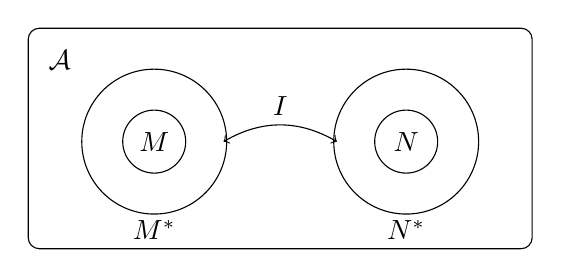
\begin{tikzpicture}[scale=.8]
\draw[rounded corners] (0,0) rectangle (8,3.5);
\draw (2,1.7) circle (1.15);\draw (6,1.7) circle (1.15);
\draw (2,1.7) circle (.5);\draw (6,1.7) circle (.5);
\node at (.5,3){$\mathcal A$};\node at (2,1.7){$M$};\node at (6,1.7){$N$};
\node at (2,.3){$M^*$};\node at (6,.3){$N^*$};
\draw[<->] (3.1,1.7) to[bend left] node[above]{$I$} (4.9,1.7);
\end{tikzpicture}
\end{center}
The crucial observation is that this coding language has an $L$-sentence
$D_1$ saying that the distinguished $M$-sort satisfies $E$ while the
$N$-sort does not; here relativization is used. It also has first-order
conditions $D_2$ saying that the internal relation $I$ is a nonempty
back-and-forth family of partial isomorphisms. By the
L\"owenheim--Skolem Property these conditions have a countable model
$\mathcal A_0$ with distinguished substructures $M_0,N_0$ satisfying
$M_0\models_LE$, $N_0\not\models_LE$, and $M_0\simeq_pN_0$.
But countable partially isomorphic structures are isomorphic, by the
usual alternating enumeration and back-and-forth construction.
This contradicts isomorphism invariance of the normal logic.
\end{proof}

\begin{lemma}[Bounded quantifier-rank dependence; lindstrom-proof]
Let $E\in L(\mathcal L)$ with $\mathcal L$ finite and relational.
Suppose there is $n$ such that whenever $M\equiv_nN$ and
$M\models_LE$, also $N\models_LE$. Then $E$ is equivalent to a
first-order sentence.
\end{lemma}
\begin{proof}
Up to logical equivalence there are only finitely many first-order
sentences of quantifier rank at most $n$ in the finite language.
For a fixed $M$, let $D_M$ be the conjunction of those true in $M$,
choosing one representative of each equivalence class. Thus
$N\models D_M$ if and only if $N\equiv_nM$.
Put
\[
D=\bigvee\{D_M:M\models_LE\}.
\]
This disjunction is finite up to logical equivalence.
If $N\models D$, it satisfies some $D_M$ with $M\models_LE$, and the
hypothesis gives $N\models_LE$. Conversely, if $N\models_LE$,
$D_N$ is one of the disjuncts and $N\models D_N$, so $N\models D$.
Hence $\operatorname{Mod}_L(E)=\operatorname{Mod}(D)$.
\end{proof}

\begin{theorem}[Lindstr\"om's Theorem]
A normal abstract logic having Compactness and the downward
L\"owenheim--Skolem Property is equivalent in expressive power to
first-order logic.
\end{theorem}
\begin{proof}
By the lemma it suffices to show that for each $E\in L(\mathcal L)$
in a finite language there is $n$ such that $M\equiv_nN$ implies that
$M$ and $N$ agree on $E$. The finite relational-language back-and-forth
characterization lets us replace $M\equiv_nN$ by
$I_n(\emptyset,\emptyset)$.

Suppose to the contrary that for every $n$ there are $M_n,N_n$ with
$I_n(\emptyset,\emptyset)$ but $M_n\models_LE$ and
$N_n\not\models_LE$. By isomorphism invariance their interpretations
of constants may be taken to be the same objects. There are finitely
many atomic sentences, so, passing to a subsequence if needed, take
the structures to agree on these atomic sentences.
Let $M$ be the union of the $M_n$, with different copies otherwise
disjoint, so each is a substructure of the resulting relational
structure. As in the preceding proof, form $M^*$ by adjoining the
finite-sequence sort and the concatenation predicates. Do the same for
$N_n,N,N^*$.

Build a larger structure $\mathcal A$ whose domain contains those of
$M^*,N^*$ and the natural numbers with their discrete ordering.
Use new predicates for all the sorts and predicates $R,S$ coding the
indexed substructures, so that
\[
M_n=\{a\in M:R(a,n)\},\qquad
N_n=\{b\in N:S(b,n)\}.
\]
The same sort-indexing predicates apply to sequences lying in a given
$M_n$ or $N_n$. Add a ternary predicate $J$ for the bounded
back-and-forth relations:
\[
J(n,\mathbf a,\mathbf b)\quad\Longleftrightarrow\quad
I_n(\mathbf a,\mathbf b).
\]
In the expanded language one can state the discrete order axioms
(first element, no last element), the relativized assertions
$M_n\models_LE$, $N_n\not\models_LE$, and the recursive conditions
for $J$ as an $L$-sentence $D$. These conditions hold in $\mathcal A$.

Compactness supplies a model $\mathcal A^*$ of these conditions with a
nonstandard element $n^*$ of the order: add a constant required to
exceed every standard natural-number stage, and use finite satisfiability.
Inside $\mathcal A^*$ are therefore substructures
$M_{n^*},N_{n^*}$ with
\[
M_{n^*}\models_LE,\qquad N_{n^*}\not\models_LE.
\]
Define a family of correspondences on their finite tuples by
\[
(\mathbf a,\mathbf b)\in\mathcal I
\quad\Longleftrightarrow\quad
J(n^*-k,\mathbf a,\mathbf b),
\]
where $k$ is the common (standard finite) tuple length.
For every standard $k$, $n^*-k>0$. Consequently the recursive clauses
for $J$ permit a further extension in either structure, and this family
witnesses $M_{n^*}\simeq_pN_{n^*}$.
The preceding theorem makes these structures $L$-equivalent, contrary
to their different values on $E$. Thus a finite $n$ exists, and the
lemma supplies a first-order equivalent of every $E$.
Normality already includes first-order expressive power, so the two
logics are equivalent.
\end{proof}
